% !TEX encoding = UTF-8
% !TEX TS-program = pdflatex
% !TEX root = ../tesi.tex
% !TEX spellcheck = it-IT

%**************************************************************
\chapter{Il progetto di stage}
\label{cap:progetto-stage}
%**************************************************************

% \intro{Brevissima introduzione al capitolo}\\

%**************************************************************
\section{Introduzione al progetto}
Il progetto sul quale è stato incentrato il mio stage presso Mediana S.r.l.u. è stato \textbf{NPS EBS}, ovvero una variante del già citato CSIndex per il cliente \textbf{E.ON Business Services} (EBS). Il nome NPS si rifà invece alla nota tipologia di indagine \textbf{Net Promoter Score} nella sua variante dedicata ai dipendenti (eNPS).

\section{Il concetto eNPS}
\label{concetto eNPS}
L'idea di base nasce da una semplice considerazione: ascoltare il giudizio del cliente non è sufficiente a migliorare nel lungo termine la \gls{customer experience}, ma è necessario considerare anche le opinioni ed il \textit{feedback} dei propri dipendenti. Quest'ultimi sono coloro che osservano giornalmente le reazioni dei clienti, ma anche coloro che gestiscono le interazioni e che comprendono e conoscono i processi operativi, avendo il potere di formare le esperienze dei clienti. Quindi se l'esperienza dei dipendenti è negativa, questi finiranno per mettere a serio rischio la relazione con i clienti. \\
Per questo motivo, per implementare un corretto programma che risponda a queste esigenze, è necessario definire innanzitutto una metrica chiara. Una delle più utilizzate è per l'appunto l'eNPS (Employee Net Promoter Score), apprezzabile sia per la sua semplicità che per la sua immediatezza. Infatti come per la metodologia NPS classica, ideata per ascoltare le opinioni del cliente, si basa sulle risposte date ad una semplice domanda:
\begin{center}
\emph{Su una scala da 0 a 10, con quale probabilità consiglieresti questa azienda come posto di lavoro?}
\end{center}
I dipendenti possono essere quindi suddivisi in tre categorie:
\begin{itemize}
\item \textbf{Promotori}: coloro che hanno dato un voto pari a 9 o 10;
\item \textbf{Passivi}: coloro che hanno dato un voto pari a 7 o 8;
\item \textbf{Detrattori}: coloro che hanno dato un voto che va da 0 a 6.
\end{itemize}
A questo punto il punteggio NPS viene calcolato, come rappresentato anche nella \hyperref[NPS]{Figura 2.1} secondo questa formula:
\begin{center}
$ NPS = \%Promotori - \%Detrattori $
\end{center}

\begin{figure}[ht]
\begin{center}
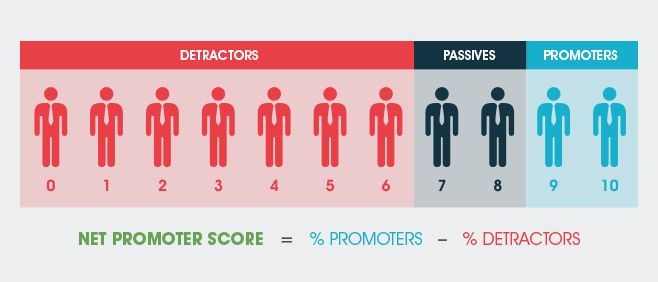
\includegraphics[scale=0.55]{NPS}
\caption{Net Promoter Score (NPS)}
\label{NPS}
\end{center}
\end{figure}
\FloatBarrier

In aggiunta a questo quesito non deve però mancare anche un'altra domanda a risposta aperta:
\begin{center}
\emph{Quali sono le ragioni del tuo voto?}
\end{center}
Solo in questo modo infatti è davvero possibile riuscire a cogliere le indicazioni e consigli che i dipendenti vorranno dare. 
%Infatti delle semplici domande a risposta chiusa costringono i rispondenti a schemi prefissati che rispecchiano sì il modo di vedere dell’organizzazione ma che non colgono di certo gli aspetti non ancora esplorati.

\section{Il progetto NPS EBS}
Sulla base di quanto espresso nella \hyperref[concetto eNPS]{Sezione 2.2}, l'E.ON Business Services (EBS) di Hannover (Germania) (logo nella \hyperref[EON]{Figura 2.2}) ha richiesto a Mediana S.r.l.u. un applicativo per gestire \textit{web survey} in moda da calcolare l'eNPS ed analizzare i dati in base ai \textit{feedback} raccolti.

\begin{figure}[ht]
\begin{center}

\includegraphics[height=45pt]{eon}
\caption{Logo del committente E.ON}
\label{EON}
\end{center}
\end{figure}

\subsection{Tipi di indagine}
Sono previsti tre differenti approcci nell'effettuare le indagini d'interesse:
\begin{itemize}
\item \textbf{Top-down}: permette ai dipendenti delle diverse sedi di EBS di dare un giudizio sui vari reparti che lo costituiscono (\textit{Human Resource}, \textit{Finance}, \acrshort{it}, ecc.) o sui servizi interni offerti;
\item \textbf{Bottom-up}: permette ai dipendenti di E.ON, che hanno avuto un interazione con EBS per risolvere alcuni problemi, di dare un giudizio sulla qualità del lavoro che in quel particolare caso è stato svolto;
\item \textbf{Passive}: permette a tutti i dipendenti di E.ON di dare un giudizio generico e anonimo su EBS.
\end{itemize}
Per quanto riguarda i primi due approcci la prima operazione da cui partire per poter effettuare le indagini d'interesse è il recupero delle informazioni sui potenziali intervistati. Per poter scegliere i contatti con i quali interagire è necessario prima caricare i dati anagrafici dei dipendenti.
% e gli eventuali \textit{touchpoint}.
Questa operazione, che viene effettuate dall'amministratore quando necessaria, fa si che il sistema NPS memorizzi o aggiorni, all'interno del proprio \textit{database}, i dati dei vari contatti che successivamente potranno essere selezionati nel caso l'esigenza dell'indagine lo richieda. \\
Terminata la fase di \textit{upload} dei contatti si passa appunto alla fase di selezione dove il responsabile dell'indagine può scegliere le persone, che verranno poi interpellate tramite una \textit{survey}, caricando nell'apposita sezione un \textit{file} CSV che rispetti la struttura concordata con il cliente oppure selezionandoli da una lista all'interno dell'applicativo. Queste prima di essere confermate dovranno superare i criteri dell'algoritmo, che permettono di evitare il verificarsi di situazioni che potrebbero infastidire gli intervistati. \\
Nello specifico i controlli fatti sono i seguenti:
\begin{itemize}
\item \textbf{Quality Control}: nel caso vengano selezionati dei contatti non presenti nel sistema o presenti più volte nello stesso \textit{file} CSV o quant'altro, questi vengono scartati;
\item \textbf{Blacklist}: nel caso vengano selezionati dei contatti che erano stati inseriti in precedenza nella \textit{blacklist} (per esempio quelli che hanno fatto richiesta di non voler più essere contattati per le indagini), questi vengono scartati;
\item \textbf{Obsolescenza}: nel caso vengano selezionati contatti che hanno ricevuto già una \textit{survey} nel breve periodo (predefinito) questi vengono scartati;
\item \textbf{Undercapacity}: nel caso venga selezionato un numero minore di contatti rispetto al numero minimo di \textit{survey} richieste per un così detto \textit{target group/touchpoint} (l'obbiettivo di studio di un indagine), tutti i contatti vengono scartati;
\item \textbf{Overcapacity}: nel caso venga selezionato un numero maggiore di contatti appartenenti ad una particolare sezione di EBS 
%(definiti nell'applicativo come \textit{Resolver Group Team}) 
rispetto al numero massimo di \textit{survey} gestibili da ogni responsabile di queste aree, vengono scartati i contatti che hanno una priorità minore rispetto a quella degli altri.
\end{itemize}
L'applicativo procede automaticamente con l'invio delle \textit{e-mail}, le cui parti sono personalizzabili dagli amministratori del sistema in un'apposita sezione del programma. In ogni \textit{e-mail} è presente un \textit{link} ad una \textit{web survey} che contiene, in base all'approccio, le rispettive domande NPS nelle quali gli intervistati possono sia dare un voto che giustificare, se essi lo vorranno, la risposta data in un apposito spazio. \'E infine presente un \textit{flag} che permette di dare il consenso di essere ricontattati per una così detta \textbf{second call}, che sarà utile per capire più approfonditamente le ragioni del giudizio che è stato dato.
In ogni momento, da quando un destinatario di queste \textit{e-mail} inizia a compilare una \textit{survey}, può decidere di interrompere momentaneamente la sua compilazione pur non avendola completata e ultimarla soltanto in un secondo momento. Se la \textit{survey} scade e non è stata ancora completata allora viene chiusa e tutti i dati parziali che erano stati immessi vengono cancellati; mentre se fin dall'inizio viene ignorata allora il sistema invia una nuova \textit{e-mail} di promemoria. Il periodo di attesa prima dell'invio della \textit{e-mail} di promemoria e la data di scadenza di una \textit{survey} possono essere configurate in una schermata apposita dell'applicativo NPS. I \textit{feedback} vengono dunque registrati nel sistema e viene tenuta traccia di tutti i dettagli dall'invio delle \textit{e-mail} fino alla conferma di compilazione completata, quindi non solo le risposte date ma anche lo stato delle \textit{survey} e le date di interesse come quelle di emissione e quelle nel quale vengono confermati i \textit{feedback} dai dipendenti.\\
L'approccio \textbf{Passive} permette invece a chiunque abbia accesso all'EBS \gls{intranet} di accedere tramite un apposito \textit{link} ad una \textit{web survey} che, a differenza degli altri due approcci appena visti, darà la possibilità di rispondere al quesito NPS in modo del tutto anonimo, presentandosi visivamente come nella \hyperref[Passive]{Figura 2.3}. Per questo motivo il sistema è in grado di riconoscere l'origine diversa del feedback registrandolo in modo che esso sia poi distinguibile dagli altri. Nel caso si volesse essere ricontattati per una \textbf{second call}, basterà comunque inserire in un' apposita sezione della \textit{survey} l'identificativo con il quale si è registrati all'interno dell'applicazione NPS, perdendo però in questo modo l'anonimato. 

\begin{figure}[ht]
\begin{center}
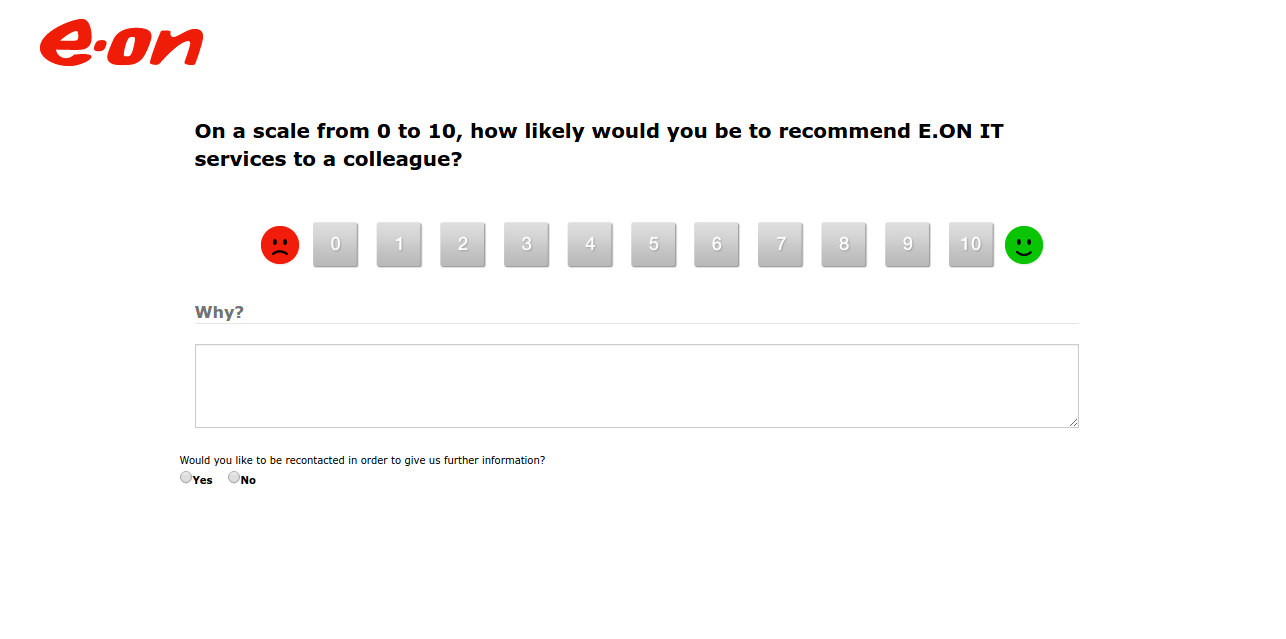
\includegraphics[scale=0.34]{PassiveSurvey}
\caption{Esempio di survey utilizzando un approccio Passive}
\label{Passive}
\end{center}
\end{figure}
\FloatBarrier

\subsection{Categorizzazione}

Per ogni \textit{feedback} raccolto dalle \textit{survey} viene data la possibilità di condurre una categorizzazione su quattro livelli (opzionali) in una maschera dedicata:\begin{enumerate}
\item \textbf{Type}: categoria che descrive il tipo di \textit{feedback}, ovvero in concreto se questo corrisponde a una segnalazione negativa, un complimento o un suggerimento;
\item \textbf{Class}: categoria che descrive in modo generico il contenuto del \textit{feedback} (per esempio "sostituzione hardware");
\item \textbf{Topic}: sotto-categoria legata strettamente a quella esposta nel punto precedente che la descrive più nel dettaglio (prendendo per buono l'esempio "sostituzione hardware" qui potrebbe essere "laptop","schermo PC","cellulare",ecc.);
\item \textbf{Reasons}: categoria che descrive le motivazioni che hanno spinto a rilasciare quel voto.
\end{enumerate}
Il responsabile di ogni sezione di EBS potrà visualizzare e quindi classificare, nel modo definito precedentemente, soltanto i \textit{feedback} della propria area di competenza. Nella stessa maschera, visibile nella \hyperref[Categorization]{Figura 2.4}, sarà inoltre possibile riportare per iscritto gli eventuali chiarimenti effettuati tramite le \textit{call}, che potranno a loro volta essere categorizzate.

\begin{figure}[h!]
\begin{center}
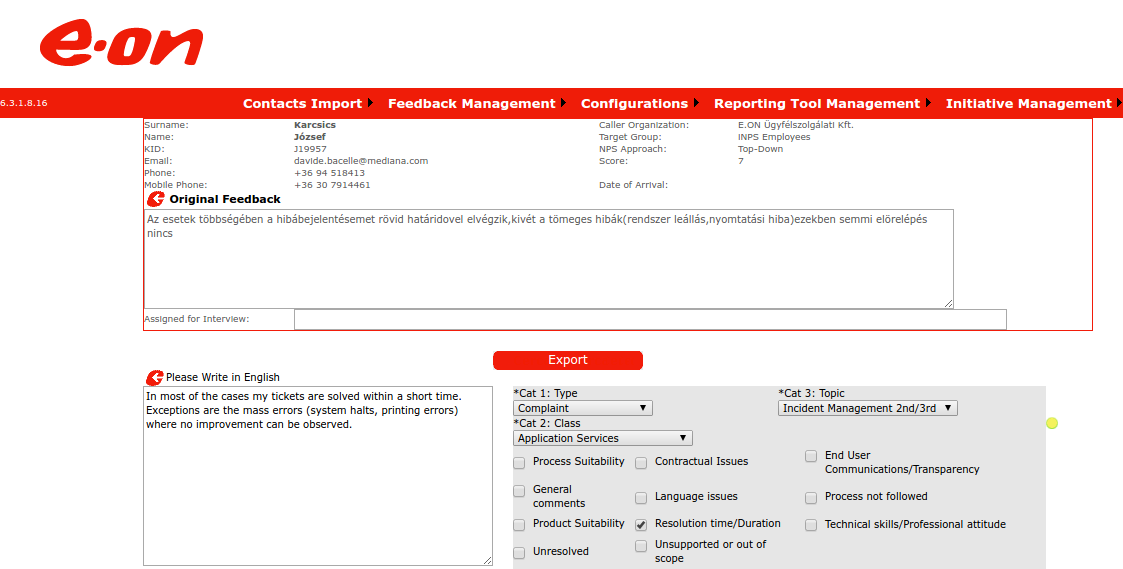
\includegraphics[scale=0.34]{FeedbackCategorized}
\caption{Esempio di feedback categorizzato}
\label{Categorization}
\end{center}
\end{figure}
\FloatBarrier

In questa sezione infine ogni \textit{feedback} può assumere tre stati differenti:
\begin{itemize}
\item \textbf{To Do}: \textit{feedback} rilasciati che non sono ancora stati categorizzati dalla persona addetta a tale operazione;
\item \textbf{Draft}: \textit{feedback} categorizzati solo in parte o comunque da rivedere prima di essere salvati definitivamente;
\item \textbf{Categorized}: \textit{feedback} categorizzati in modo definitivo e quindi non più modificabili.
\end{itemize}

\subsection{Reportistica}
\label{reporting tool}
I punteggi e i \textit{feedback} che sono stati memorizzati all'interno del \textit{database}, possono essere visualizzati tramite grafici che permetto all'utente di analizzare le varie statistiche nel modo più semplice possibile. \\
Esistono tre tipologie differenti di grafico:
\begin{itemize}
\item \textbf{Grafico a linee}: indicato per analizzare l'andamento temporale di una particolare statistica;
\item \textbf{Grafico a barre}: indicato per analizzare la distribuzione di una particolare statistica;
\item \textbf{Grafico a torta}: indicato per avere una visione d'insieme di una particolare statistica (esempio nella \hyperref[torta]{Figura 2.5}).
\end{itemize}

\begin{figure}[h!]
\begin{center}
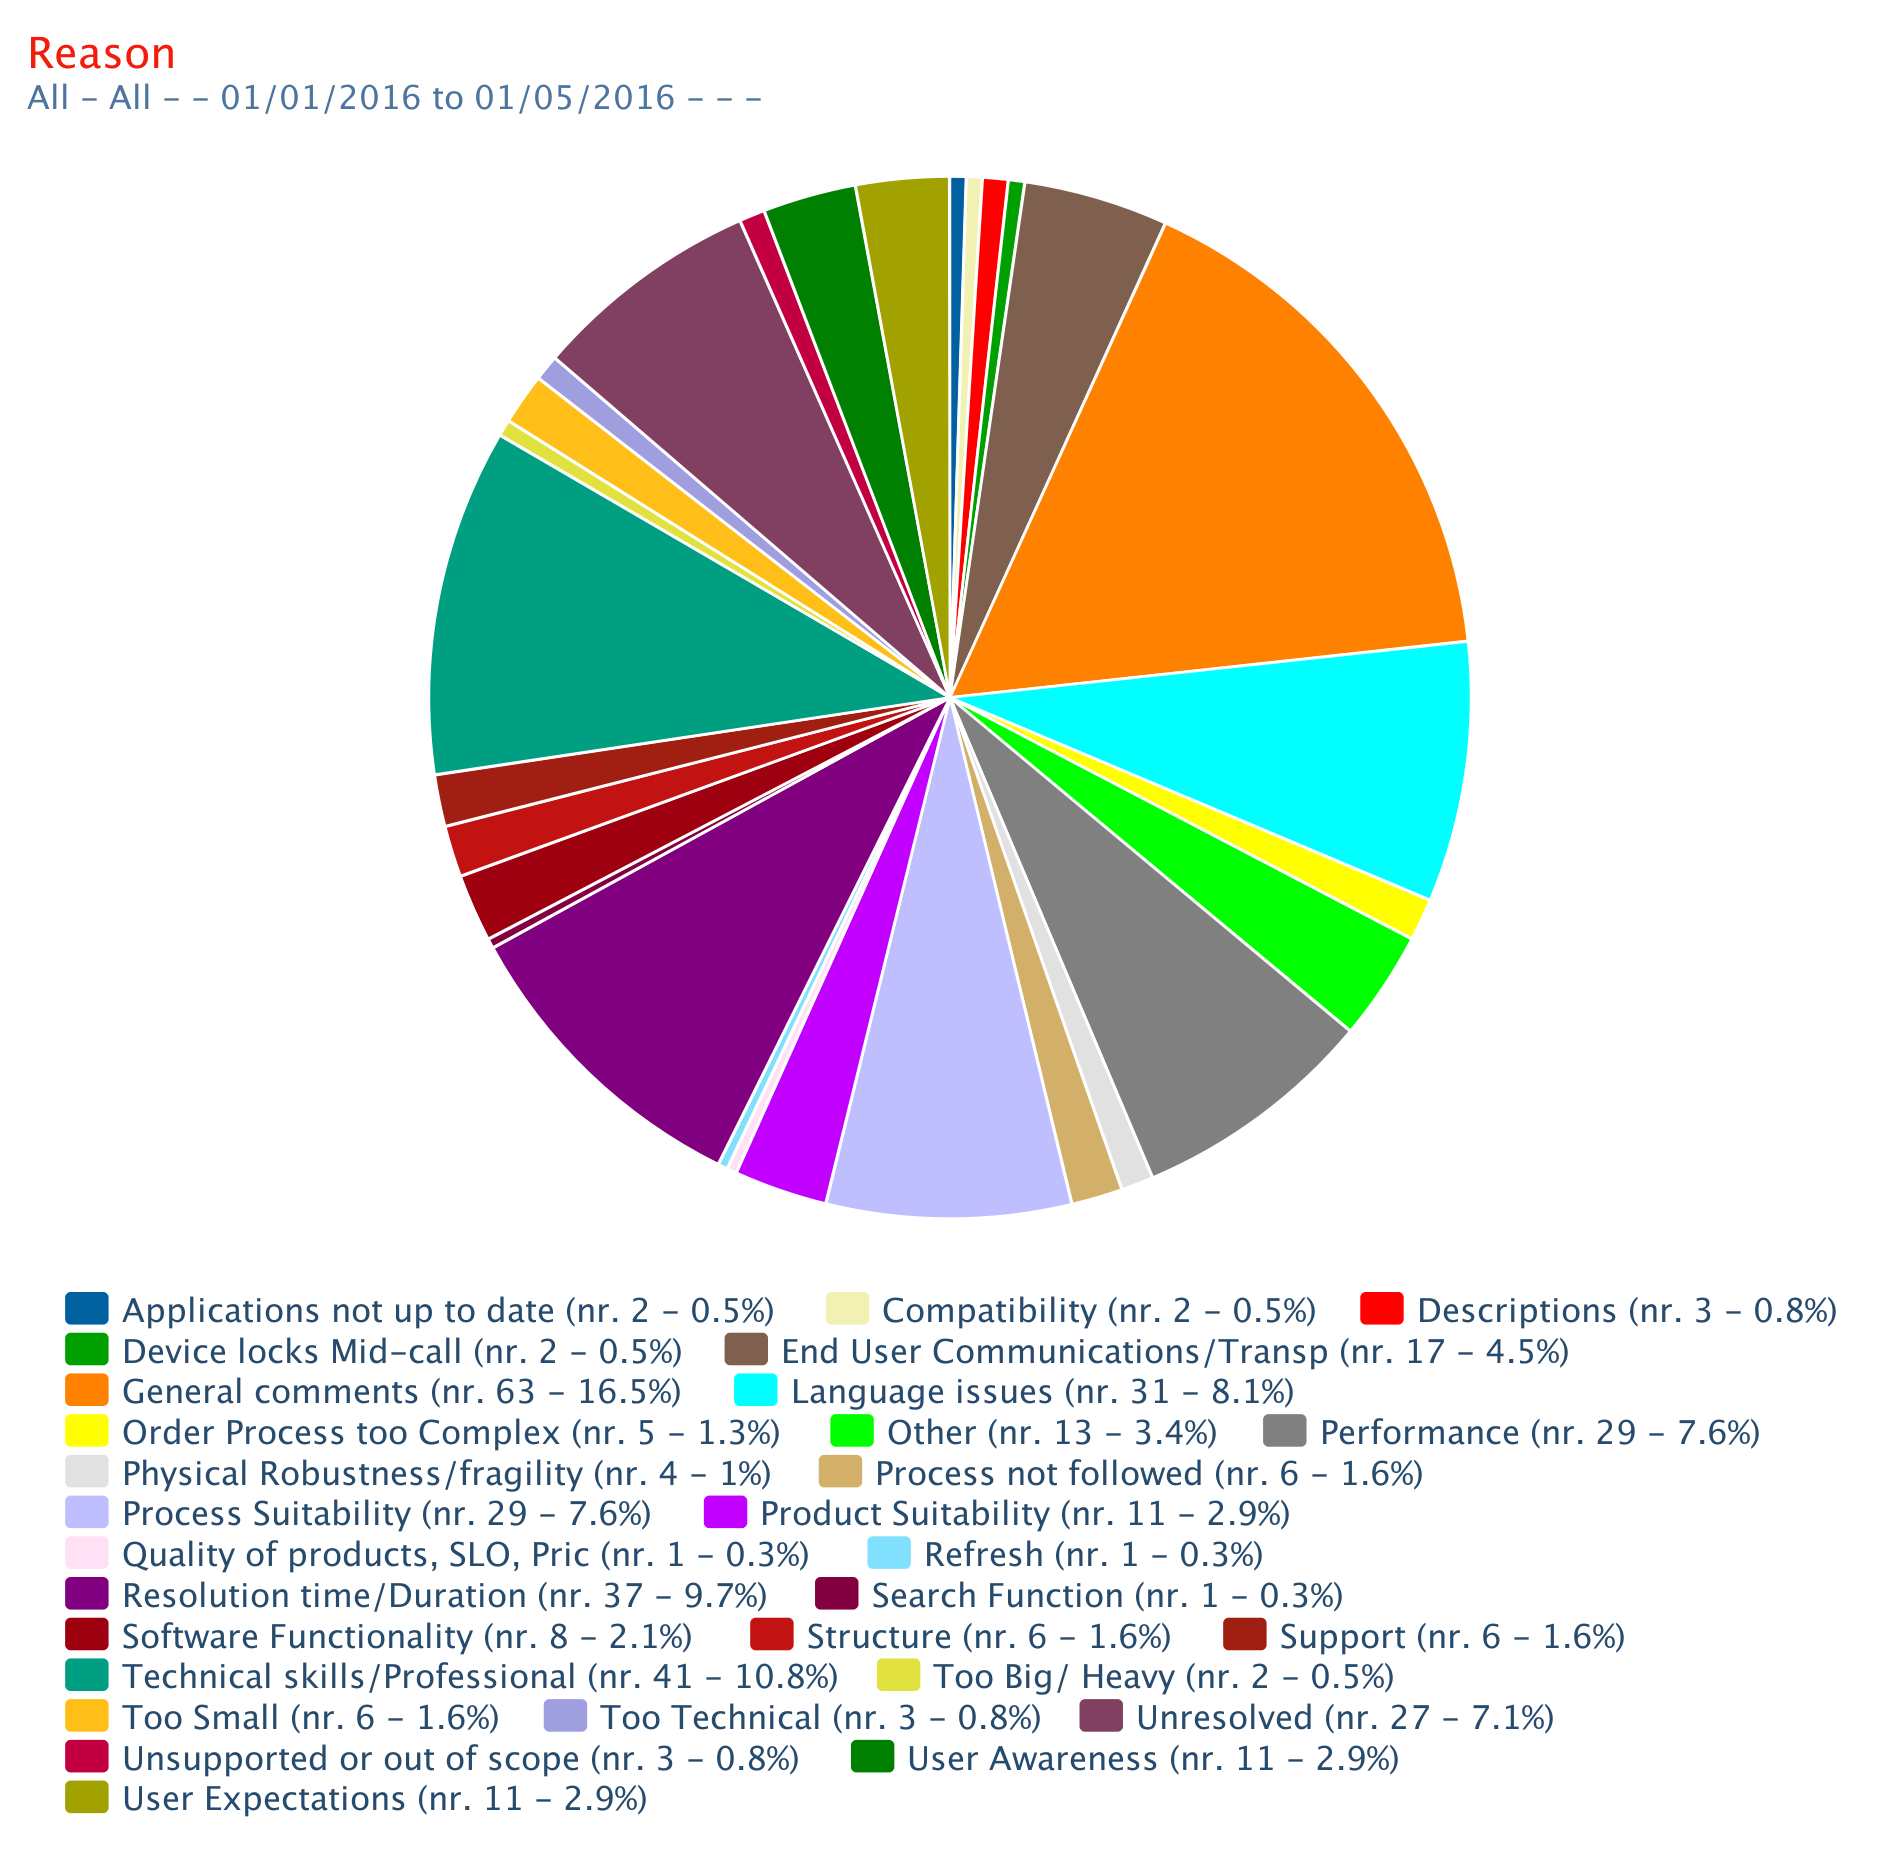
\includegraphics[scale=0.2]{GraficoTorta}
\caption{Esempio di grafico a torta}
\label{torta}
\end{center}
\end{figure}
\FloatBarrier

Questa pagina del programma NPS mette inoltre a disposizione le seguenti funzionalità e caratteristiche: 
\begin{itemize}
\item \textbf{Filtri}: utili per selezionare soltanto i dati di reale interesse, per esempio permettono di selezionare il periodo, la granularità, l'approccio delle \textit{survey} e le categorie dei \textit{feedback};
\item \textbf{Stampa e Download}: è possibile esportare il grafico in formato JPEG, PNG, SVG (formato vettoriale) e PDF oppure stamparlo direttamente dalla pagina web;
\item \textbf{Legenda dinamica}: cliccando le voci della legenda si possono togliere/aggiungere dal grafico i dati selezionati;
\item \textbf{Labels}: passando sopra con il mouse nelle diverse parti che compongono un grafico, è possibile ottenere informazioni dettagliate su queste;
\item \textbf{Zoom}: strumento che permette di visualizzare il grafico ingrandito in una finestra \textit{pop-up};
\item \textbf{Chiusura/Apertura Grafico}: strumento che permette di nascondere il grafico all'interno della pagina (tramite lo stesso bottone è poi possibile riaprirlo).
\end{itemize}

\subsection{Iniziative}
L'iniziativa è un'azione intrapresa da EBS con lo scopo di migliorare la soddisfazione del suo organico. Questa è verificabile attraverso l'invio di successive \textit{survey} sullo stesso argomento.\\
La necessità di programmare una nuova iniziativa parte dall'analisi fatta in seguito
alla raccolta dei dati con le \textit{survey}.\\
Individuata la categoria bisognosa di un intervento è necessario passare
all'approfondimento dei singoli \textit{feedback} per poter capire in che modo migliorare il servizio.\\
L'iniziativa può assumere tre differenti stati:
\begin{itemize}
\item \textbf{Draft}: l'iniziativa non è ancora ben definita ed è ancora modificabile;
\item \textbf{Open}: l'iniziativa è partita e non è più modificabile;
\item \textbf{Closed}: l'iniziativa è conclusa.
\end{itemize}

Terminata la creazione di una iniziativa è possibile collegarla ai \textit{feedback} di interesse e se desiderato inviare al contatto una \textit{e-mail} che lo informa sull'iniziativa intrapresa dall'azienda per migliorare la situazione.

\subsection{Impostazioni e personalizzazioni}
Senza entrare troppo nello specifico adesso elenco le molteplici sezioni che permettono una corretta configurazione della struttura e dei parametri del sistema NPS:
\begin{itemize}
\item È possibile abilitare nuovi utenti e assegnare loro uno dei ruoli previsti all'interno del sistema, a seconda delle funzioni alle quali essi possano accedere;
\item Tutte le domande, le \textit{label} e i messaggi delle \textit{survey}, oltre al corpo e l'oggetto delle \textit{e-mail}, possono essere personalizzate per definire il testo che leggeranno gli intervistati;
\item Per verificare di aver settato nel modo desiderato le impostazioni specificate nel punto precedente, l'applicativo NPS prevede una funzione dove è possibile inviare una \textit{e-mail} con una \textit{survey} di prova a un determinato indirizzo di posta elettronica;
\item Aggiungere, modificare o eliminare il possibile contenuto delle varie categorie che permettono di classificare i \textit{feedback};
\item Configurare nuovi \textit{target group/touchpoint}, che corrispondono allo scopo per le quali vengono fatte partire le indagini d'interesse, specificando parametri come per esempio il tipo di approccio da utilizzare, il periodo di validità della \textit{survey}, le opzioni di categorizzazione possibili, ecc.
\end{itemize} 
